\documentclass[10pt,twoside,slovak,a4paper]{article}

\usepackage[slovak]{babel}
\usepackage[IL2]{fontenc}
\usepackage[utf8]{inputenc}
\usepackage{graphicx}
\usepackage{url}
\usepackage{hyperref}
\usepackage{cite}
    
\pagestyle{headings}

\title{Získavanie informácií z webu a ich relevantnosť 
\thanks{Semestrálny projekt v predmete Metódy inžinierskej práce, ak. rok 2023/2024, vedenie: Ing. Ivan Kapustík}}

\author{Marián Tovarňák\\[2pt]
	{\small Slovenská technická univerzita v Bratislave}\\
	{\small Fakulta informatiky a informačných technológií}\\
	{\small \texttt{xtovarnak@stuba.sk}}
	}

\date{\small 5. november 2023}



\begin{document}

\maketitle

\begin{abstract}
V súčasnosti je internet omnoho rozsiahlejší ako kedysi. A s tým súvisí aj množstvo dát, ktoré obsahuje. Na weboch je veľké množstvo informácií a nie všetky sú relevantné.

Je veľmi dôležité rozoznávať informácie na základe toho, či sú pravdivé alebo nepravdivé. Ďalším veľkým problémom v dnešnej dobe sú hoaxy, ktoré častokrát obsahujú nepodstatné, zavádzajúce a klamlivé informácie, ktoré nás môžu zmiasť. Je dobré vedieť ako sa takýmto nepravdivým informáciám vyhýbať a ako zabrániť ich šíreniu ďalej. 

Cieľom tohto článku je naučiť sa efektívne vyhľadávať informácie na webových stránkach z veľkých databáz, vedieť rozlišovať podstatné informácie od tých nepodstatných a ako sa vyvarovať hoaxom a zabrániť ich šíreniu ďalej.
\cite{ceri2013web} \cite{doi:10.1126/science.aap9559}

\end{abstract}



\section{Úvod} 
\label{uvod} 
V úvode si definujeme pojmy ako databáza ~\ref{databaza} a informácia ~\ref{informacia}. Tento článok sa bude hlavne venovať spôsobom, ako sa dá účinne prehľadávať internet a ako vyhľadávať informácie v obrovských online databázach. V sekcii ~\ref{pravdivost} poukáže aj na to ako efektívne rozlišovať podstatné informácie od tých nepodstatných. Zároveň v sekcii ~\ref{hoax} je vysvetlený pojem hoax a ako sa brániť pred týmito dezinformáciami a ako veľmi dôležité je zabrániť ich šíreniu ďalej. Záverečná ~\ref{zaver} časť zosumarizuje túto problematiku a poskytne zhrnutie tých najdôležitejších poznatkov z tejto oblasti.

\section{Databáza}
\label{databaza}
\subsection{Definícia}
Databáza je súbor štruktúrovaných údajov alebo informácií uložených v počítačovom systéme. Je to základný koncept v informatike a používa sa na ukladanie, organizovanie a správu údajov. 
\subsection{Web ako online databáza}
Web je taktiež databáza údajov. Používatelia môžu k tejto databáze pristupovať pomocou internetového prehliadača. Táto databáza sa používa na rôzne účely, ako je napríklad ukladanie informácií o používateľoch, produktoch alebo objednávkach v e-shope, na zber dát, ako je napríklad v prípade online dotazníkov alebo ankiet. \cite{williams2004web}

\section{Informácia} 
\label{informacia}
\subsection{Definícia}
Informácie sú podnety, ktoré majú v určitom kontexte pre svojho príjemcu význam. Údaje predstavujú súbor nespracovaných, neusporiadaných faktov, zatiaľ čo informácie sú údaje zasadené do kontextu. Informácie môžu byť prenášané prostredníctvom rôznych typov komunikácie, ako je písomná, ústna, vizuálna a zvuková. Aby sa údaje zmenili na informácie, musia byť spracované a usporiadané. \cite{webster1984longman}


\section{Ako vyhľadávať informácie na webe}
\label{vyhladavanie}
Vyhľadávanie informácií na webe možno vykonávať pomocou vyhľadávacích nástrojov, čo sú webové stránky, ktoré zhromažďujú a organizujú informácie na internete a sprístupňujú ich na vyhľadávanie. Keďže web je veľmi široká databáza údajov je mnohokrát ťažké nájsť konktrétne to, čo hľadáme. Ako teda hľadať na internete informácie efektívne? \cite{inkpen2007information}

\begin{itemize}
    \item \textbf{Kľúčové slová:\\}
    Pri vyhľadávaní používajte kľúčové slová, ktoré sú relevantné pre vašu tému. Pomôže to zúžiť okruh vyhľadávaných informácií.
    
    \item \textbf{Jednoduchosť hľadaných výrazov:\\}
    Hľadané výrazy by mali byť jednoduché. Treba sa vyhnúť používaniu príliš zložitých výrazov, ktoré vyhľadávací nástroj nemusí rozpoznať.

    \item \textbf{Používanie úvodzoviek:\\}
    Ak hľadáme konkrétnu frázu alebo konkrétne slovo, dáme daný výraz do úvodzoviek. Prehliadač nám vyhodí výsledky, ktoré sa presne zhodujú s danou frázou alebo slovom.

    \item \textbf{Pokročilé vyhľadávacie nástroje:\\}
    Väčšina prehliadačov disponuje pokročilými vyhľadávacími nástrojmi, ktoré umožňujú obmedziť vyhľadávanie podľa typu, času, alebo krajiny.
    
    \item \textbf{Klávesové skratky:\\}
    Veľmi veľkým pomocníkom sú klávesové skratky ako Ctrl+F (pre Windows) alebo Command+F (pre Mac), ktoré dokážu vyhľadať konkrétne slová alebo frázy na danej stránke.
    
    \item \textbf{Iný vyhľadávací nástroj:\\}
    V dnešnej dobe existuje veľké množstvo webových prehliadačov. Ak jeden vyhľadávač nenájde konktrétne to čo hľadáte, použite ďalší.
\end{itemize}

   Efektívne vyhľadávanie na internete si vyžaduje používanie špecifických kľúčových slov, zjednodušenie hľadaných výrazov, používanie úvodzoviek, používanie pokročilých vyhľadávacích nástrojov, vyhľadávanie na stránke, skúšanie rôznych hľadaných výrazov a používanie klávesových skratiek.

\begin{figure}
    \centering
    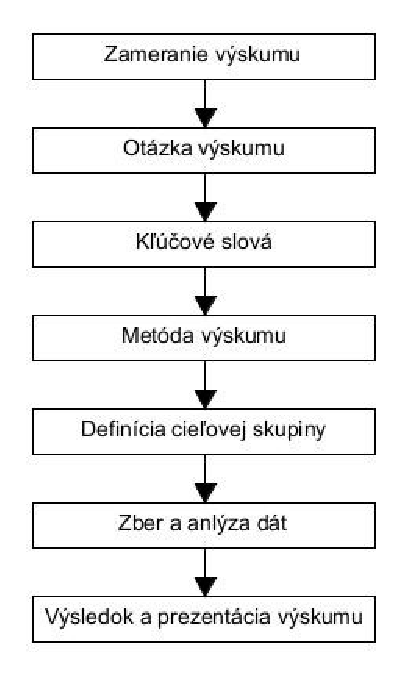
\includegraphics[width=0.4\textwidth]{tabulka1.pdf}
    \caption{Vyhľadávanie na webe}
    \label{obr1}
\end{figure}

\section{Ako rozpoznať pravdivosť informácií}
\label{pravdivost}
Identifikovať pravdivé informácie od  nepravdivých informácií môže byť veľmi náročné, najmä kvôli tomu koľko informácií sa v dnešnej dobe na webe nachádza. Ako sa vyhúť nepravdivým informáciám? \cite{de2021approaches}

\begin{itemize}
    \item \textbf{Kontrola zdrojov:\\}
    Je dôležité overovať si reputáciu zdroja, to či je daný zdroj informácii známy medzi ľudmi, či uvádza spoľahlivé správy. Treba si dávať pozor zdroje, ktoré v minulosti zverejňovali nepravdivé informácie a vyvarovať sa takýmto zdrojom.
    
    \item \textbf{Čítanie článku do úplného konca:\\}
    Často sa stáva, že článok alebo akýkoľvek text nie je dočítaný do úplného konca. To je veľká chyba, pretože nadpis daného článku alebo textu môže byť zavádzajúci. Kontext textu teda môže byť úplne odlišný ako jeho nadpis.
    
    \item \textbf{Overenie autora:\\}
    Vyhľadajte si informácie o autorovi publikovaného článku. Ak článok nemá autora, tak nie je možné považovať takýto zdroj informácií ako dôveryhodný. Netreba dôverovať ani autorom, ktorí píšu odborné články a pritom nemajú žiadne odborné znalosti v danej problematike.

    \item \textbf{Hľadanie dôkazov:\\}
    Ďalším bodom, ktorým si overíme správnosť informácií je hľadanie dôkazov alebo argumentov, ktoré poukazujú na správnosť daných tvrdení spomenutých v článku.

    \item \textbf{Kontrola dátumu:\\}
    Dôležitú úlohu zohráva aj dátum publikovania článku alebo akéhokoľvek textu, z ktorého chceme čerpať informácie. Ak je článok príliš starý je veľmi pravdepodobné, že informácie, ktoré zahŕňa už nemusia byť aktuálne. Častokrát sa stáva, že článok je prezdieľavaný a ide pri tom o starú informáciu. Spoľahnúť sa môžeme hlavne na aktuálne články.
\end{itemize}

\section{Hoax} \label{hoax}
\subsection{Definícia} 
Falošná správa (hoax) je zámerne nepravdivá a často až absurdná informáciaa vytvorená s úmyslom oklamať a zavádzať ľudí alebo niekomu uškodiť. Hoaxy môžu mať mnoho podôb, ako napríklad falošná zbierka na charitu, bombová hrozba, falošný spravodajský článok alebo často ide aj o konšpiračné teórie. \cite{irena2020fake} \cite{mcgonagle2017fake}

\subsection{Ako sa vyhýbať hoaxom}
\subsection{Ako zabrániť šíreniu hoaxov}
Užitočné stránky:\\
\url{https://hoax.sk}, \\
\url{https://hoax.cz/cze/}
\section{Záver} \label{zaver}

\bibliographystyle{plain}
\bibliography{literatura}


\end{document}